
\subsection{\texorpdfstring{The $\Zmm$ Signal Extraction}{The Z->mu mu Signal Extraction}}
\label{sec:Zmumu}

The yield of the $\Zmm$ events is determined from a fit simultaneously with the
average muon reconstruction efficiencies in the tracker and in
the muon detector, the muon trigger efficiency,
as well as the efficiency of the applied isolation requirement.
\Zmm candidates are obtained as pairs of muon candidates of different types
and organized into categories according to different requirements:
\begin{itemize}
\item $\Zmumu$: a pair of isolated global muons, further split into two samples:
\begin{itemize}
\item $\ZmumuTwoHlt$: each muons associated with an HLT trigger muon;
\item $\ZmumuOneHlt$: only one of the two muons associated with an HLT trigger muon;
\end{itemize}
\item $\Zmus$: one isolated global muon and one isolated
  stand-alone muon;
\item $\Zmut$: one isolated global muon and one isolated tracker track;
\item $\ZmumuNonIso$: a pair of global muons, of which one is isolated and the
other is nonisolated.
\end{itemize}

%The $\Zmumu$ category is also referred to as ``golden'' sample.
With the exception of the $\ZmumuOneHlt$ category, each global muon must correspond to an HLT trigger muon.
The five categories are explicitly forced to be mutually exclusive in the event
selection: if one event falls into the first category it is excluded from the second;
if it does not fall into the first category and falls into the second, it is excluded
from the third, and so on. In this way non-overlapping, hence statistically
independent, event samples are defined. The expected number of events in which more than
one dimuon combination is selected is almost negligible.
In those few cases all possible combinations are considered.

The five signal yields in each category can be written in terms of
the five unknowns, the Z signal yield $\NZtomumu$ and four efficiency terms, as follows:
\begin{eqnarray}
 \label{eqNmumuTwoHlt}
   \NmumuTwoHlt & = & \NZtomumu \effHlt^2 \effIso^2 \effTrk^2 \effSa^2,  \\
  \label{eqNmumuOneHlt}
   \NmumuOneHlt & = & 2 \NZtomumu \effHlt (1 - \effHlt) \effIso^2 \effTrk^2 \effSa^2,  \\
  \label{eqNmus}
   \Nmus & = & 2 \NZtomumu \effHlt \effIso^2 \effTrk (1 - \effTrk) \effSa^2,  \\
  \label{eqNmut}
   \Nmut & = & 2 \NZtomumu \effHlt \effIso^2 \effTrk^2 \effSa(1 -\effSa), \\
  \label{eqNmumuNonIso}
   \NmumuNonIso & = & 2 \NZtomumu \effHlt^2  \effIso (1 - \effIso)  \effTrk^2 \effSa^2.
\end{eqnarray}
The various efficiency terms in Eqs.~(\ref{eqNmumuTwoHlt}) to~(\ref{eqNmumuNonIso}),
the average efficiencies
of muon reconstruction in the tracker, $\effTrk$, in the muon detector as
a stand-alone muon, $\effSa$, the average efficiency of the isolation requirement,
$\effIso$, and the average trigger efficiency, $\effHlt$,
can be factorized because the muon selection
factorizes the requirements on the tracker and muon detector quantities separately.
Neither selection on $\chi^2$ per degree of freedom nor requirement of the muon reconstruction through the
tracker-muon algorithm is applied in order to
avoid efficiency terms that cannot be described as a product of contributions from the tracker and
the muon detector.
%We verified on Monte Carlo that the possible effects of any residual correlation
%can be either incorporated in the proper definition of the efficiencies or
%is negligible.
% Above, $\effTrk$ is
% the efficiency to reconstruct a track {\it and} to pass the track selection,
% and $\effSa$ is the efficiency to reconstruct a track in the muon detector {\it and} to pass the
% stand-alone muon selection, according to the selection described in Section~\ref{sec:muonid}.

The dimuon invariant mass spectra for the five categories are divided into
bins of different sizes, depending on the number of observed events.
The distributions of the dimuon invariant mass for the different categories can be written
as the sum of a signal peak plus a background component.


Figure~\ref{fig:zGolden36pb} shows the dimuon invariant mass spectrum for the $\Zmm$ golden events
on both a linear scale and a logarithmic scale, and Figs.~\ref{fig:zNoGold1}
and~\ref{fig:zNoGold2} show the
invariant mass distributions for the remaining categories.
The spectra are in agreement with the simulation.

\begin{figure}[hbtp]
    \begin{minipage}{73mm}
      \begin{center}
%        \resizebox{1.0\textwidth}{!}{{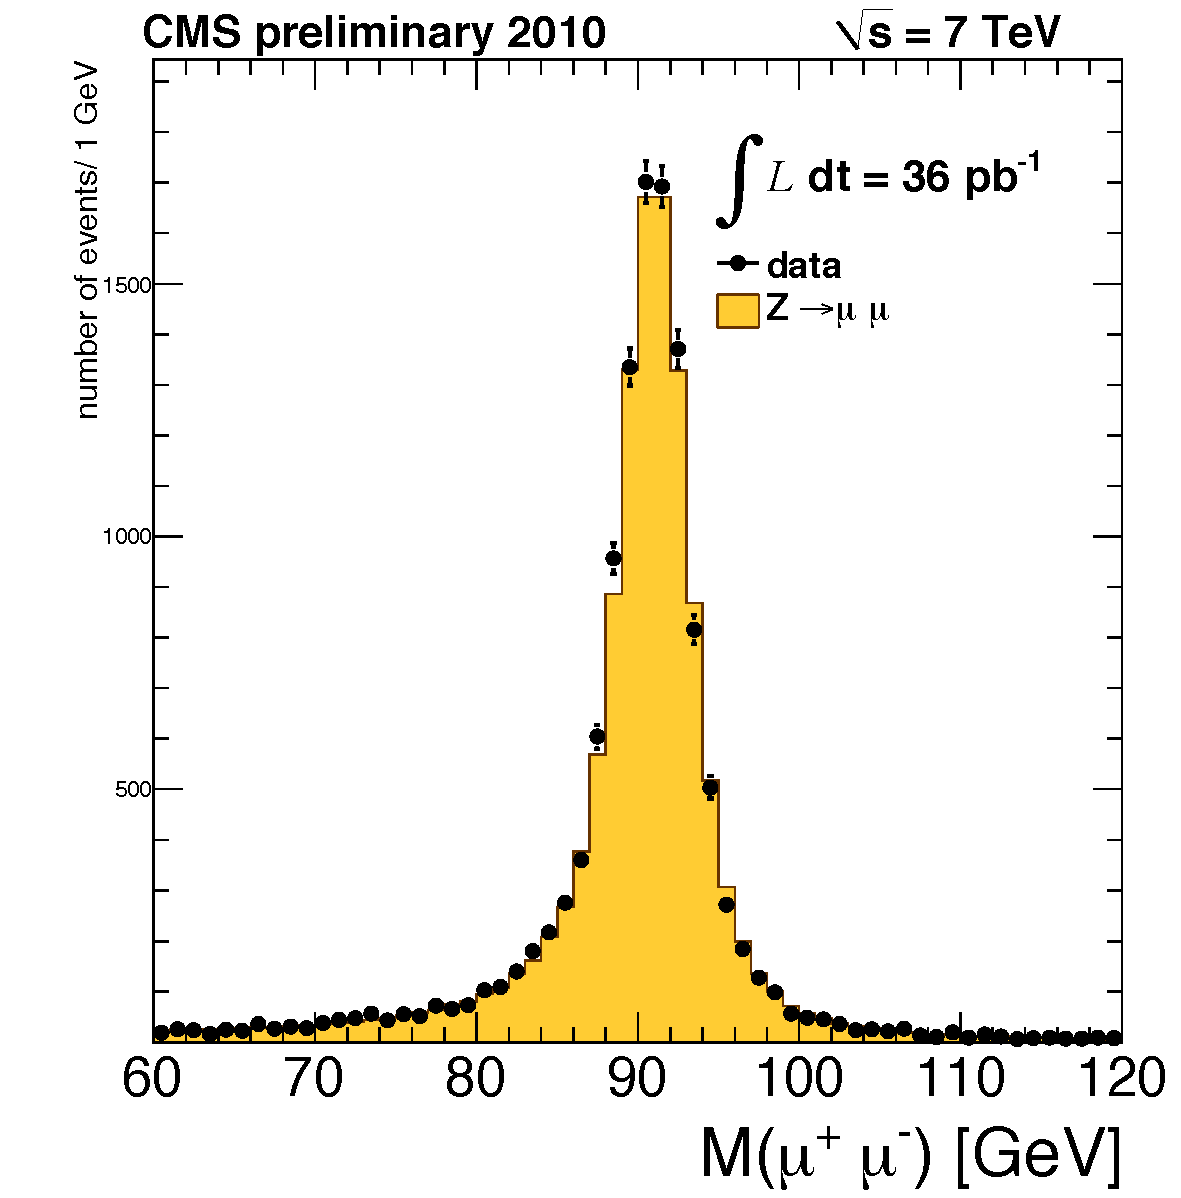
\includegraphics{figs/zGoldenLin_36pb.pdf}}}
        \resizebox{1.0\textwidth}{!}{{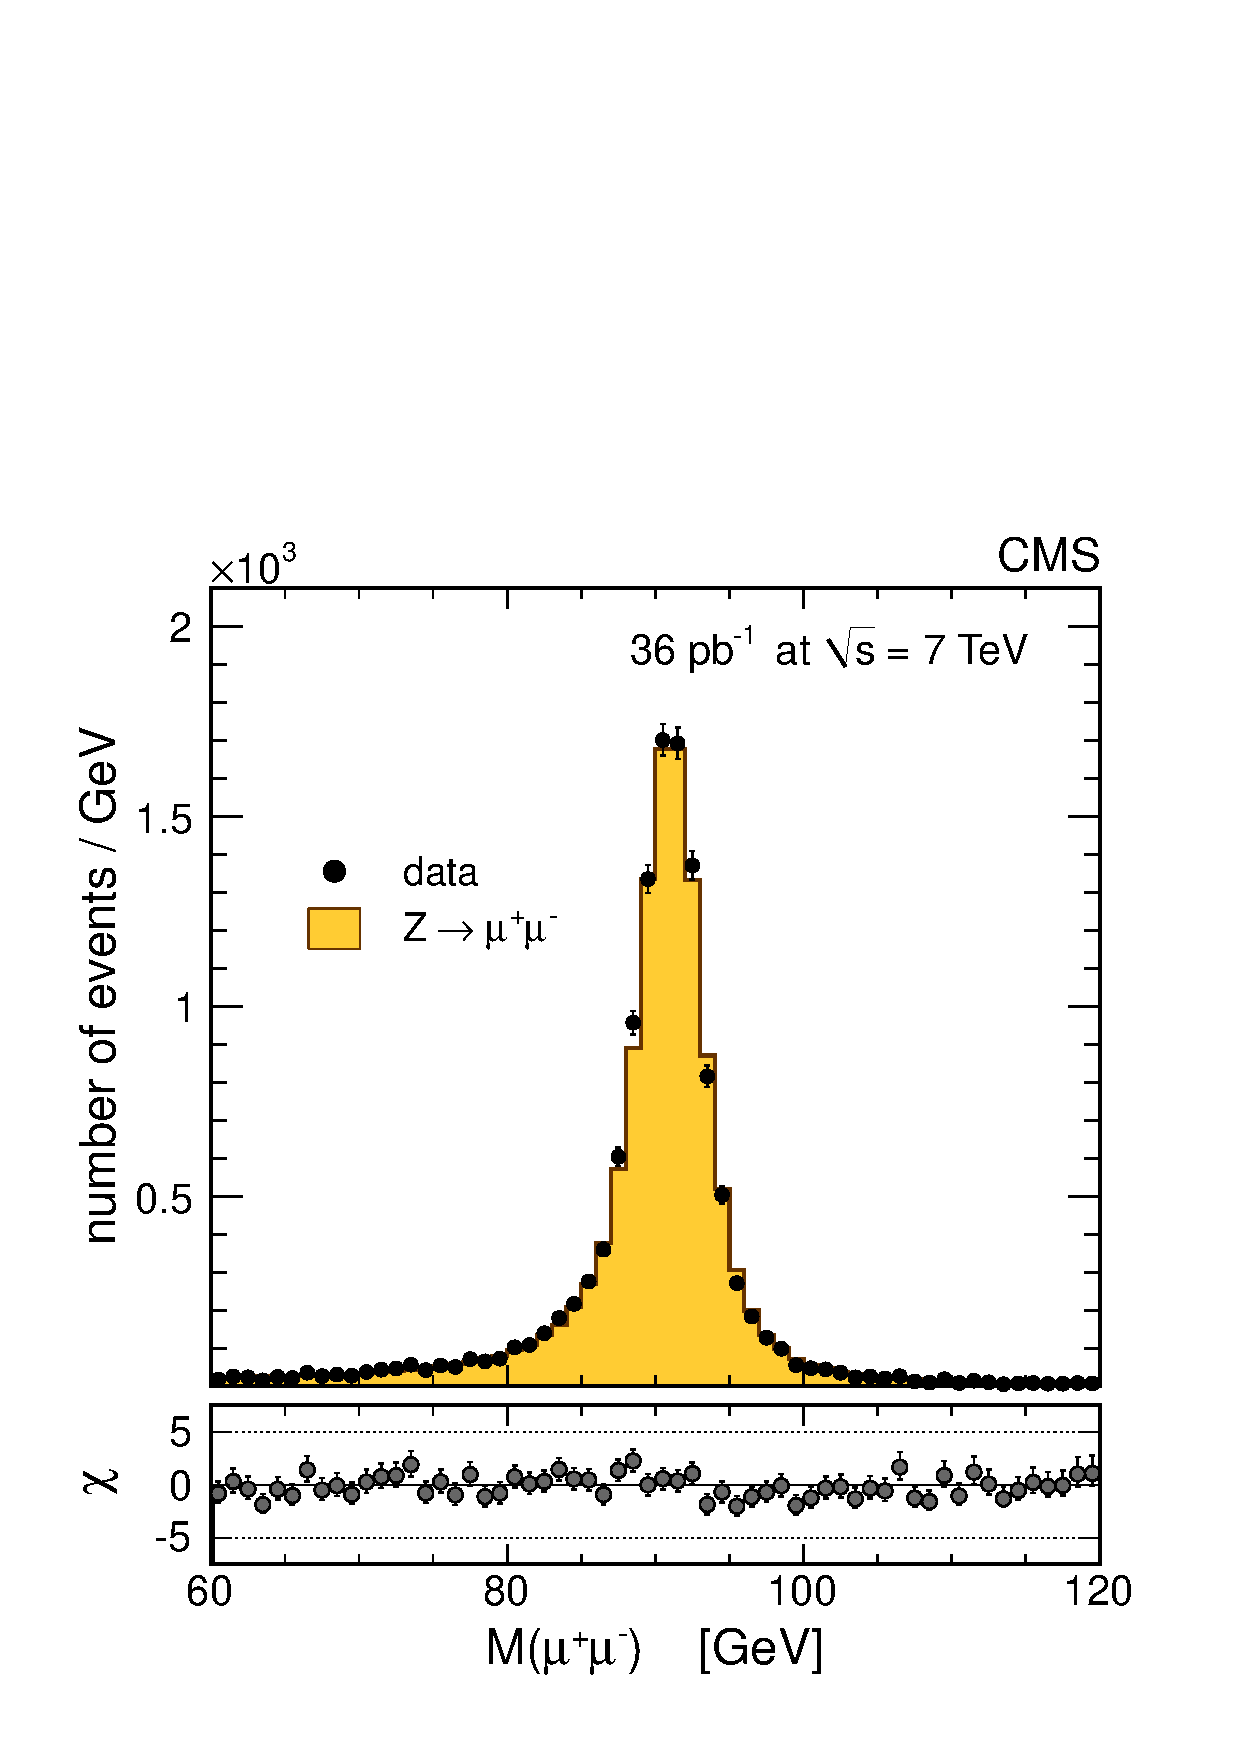
\includegraphics{figs/Zmumu_lin.pdf}}}
      \end{center}
    \end{minipage}
    \begin{minipage}{73mm}
       \begin{center}
%       \resizebox{!}{1.0\textwidth}{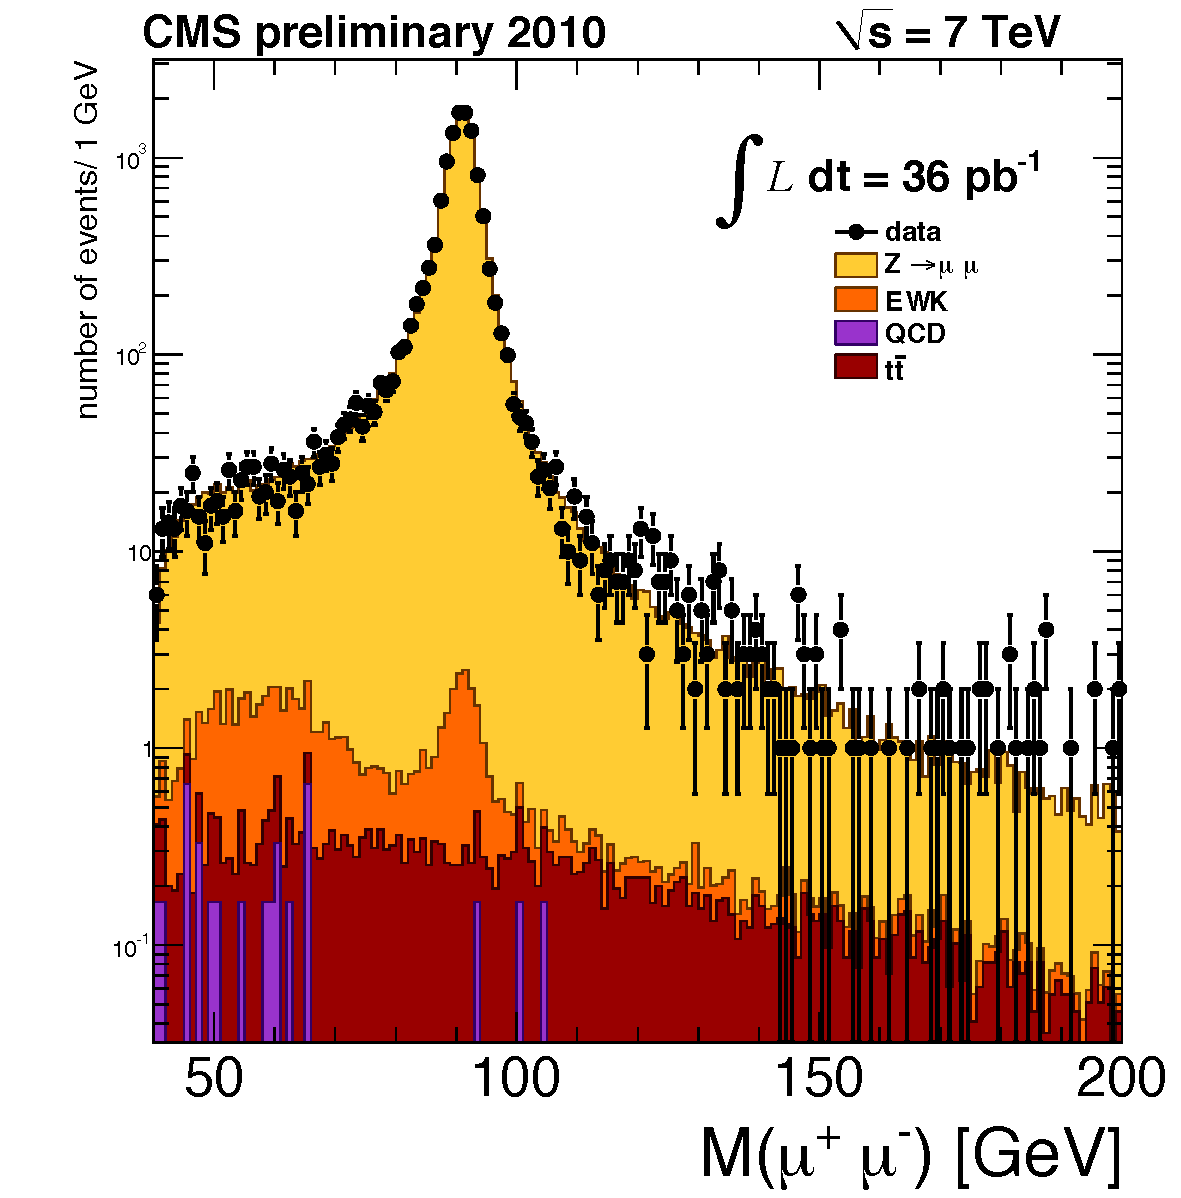
\includegraphics{figs/zGoldenLog_36pb.pdf}}
       \resizebox{!}{1.0\textwidth}{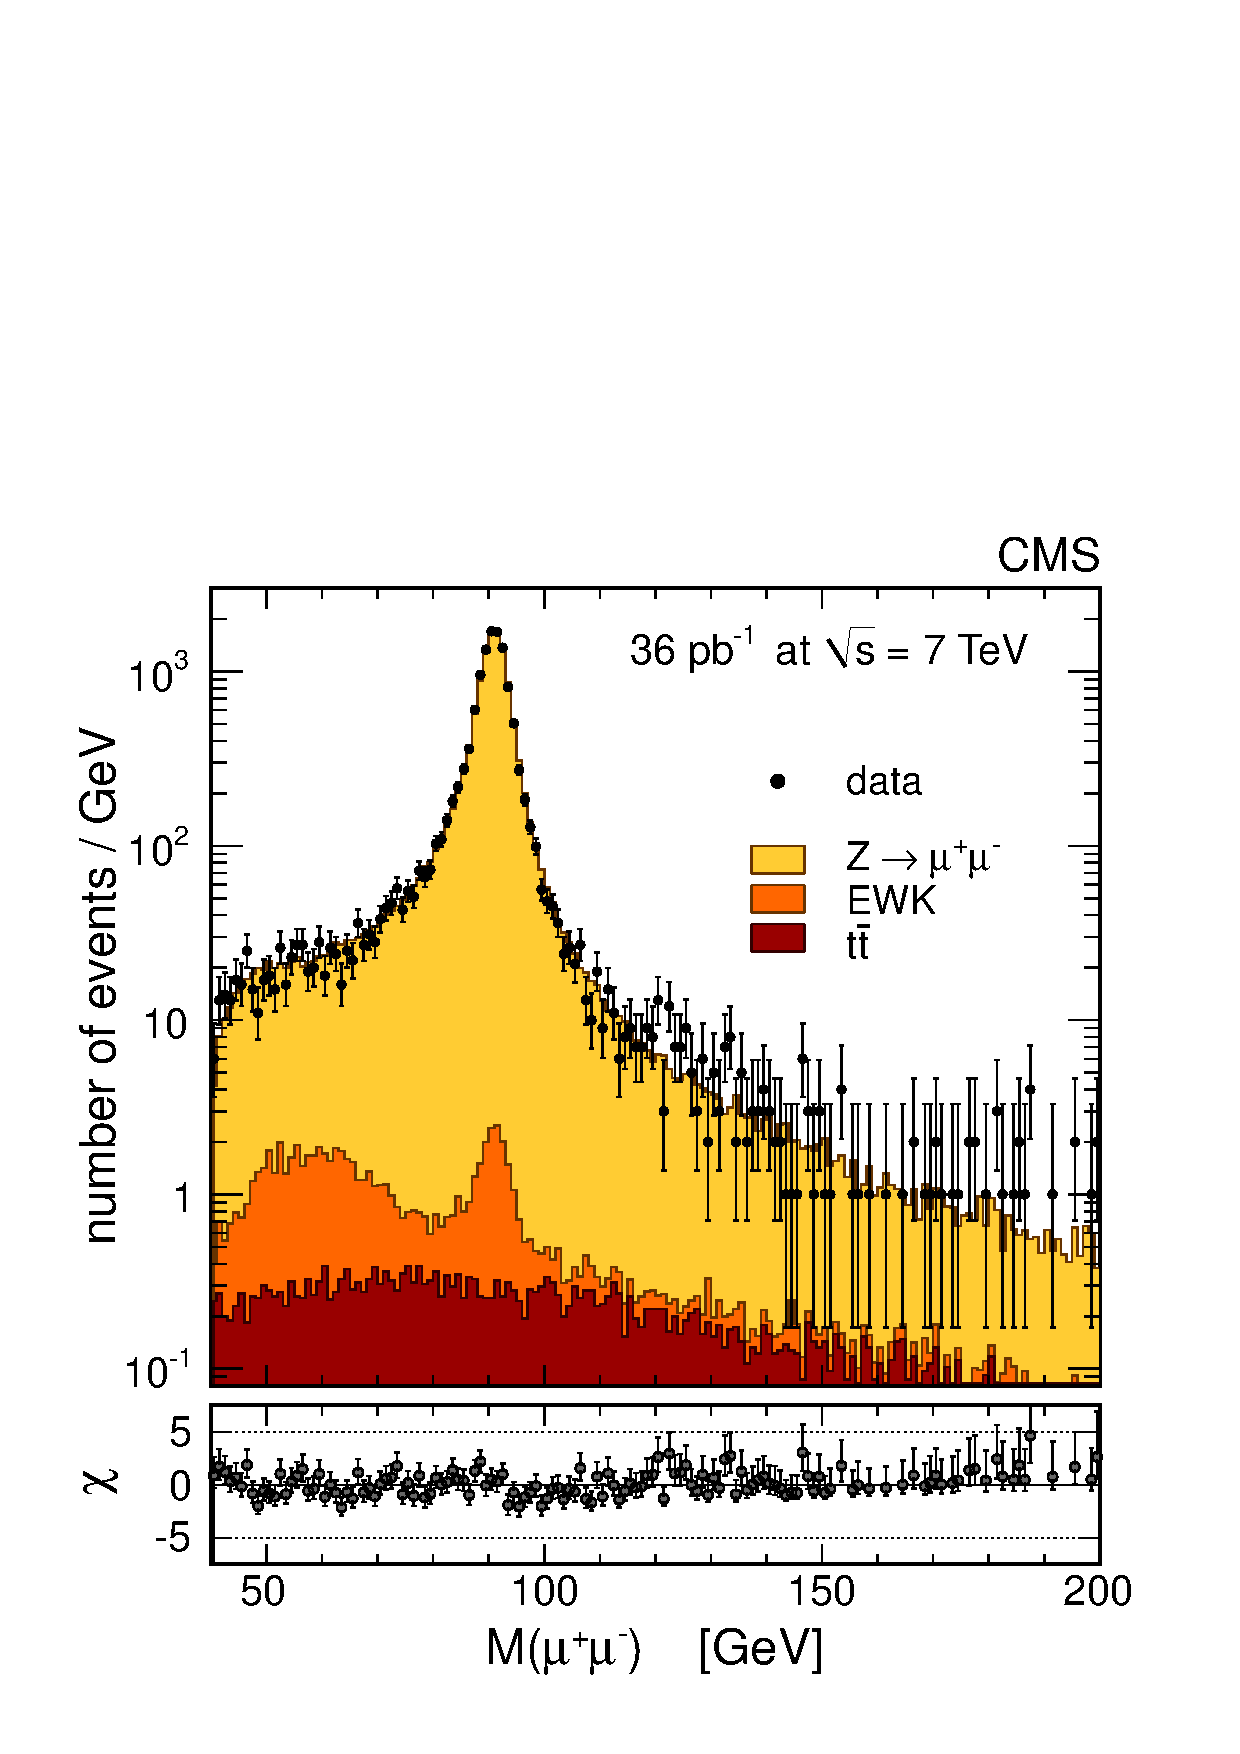
\includegraphics{figs/Zmumu_log.pdf}}
      \end{center}
    \end{minipage}
\caption{
Distributions of the dimuon invariant mass for the selected $\Zmm$ golden candidates on
a linear scale (left) and on a logarithmic scale (right).
The points with the error bars represent the data.
Superimposed are the expected distributions from simulations, normalized
to an integrated luminosity of $36$~pb$^{-1}$. The expected distributions are
the Z signal (yellow, light histogram), other EWK processes (orange, medium histogram),
and $\ttbar$ background (red, dark histogram).
Backgrounds are negligible and cannot be seen on the linear-scale plots.
}
\label{fig:zGolden36pb}
\end{figure}

\begin{figure}[hbtp]
    \begin{minipage}{73mm}
      \begin{center}
        \resizebox{1.0\textwidth}{!}{{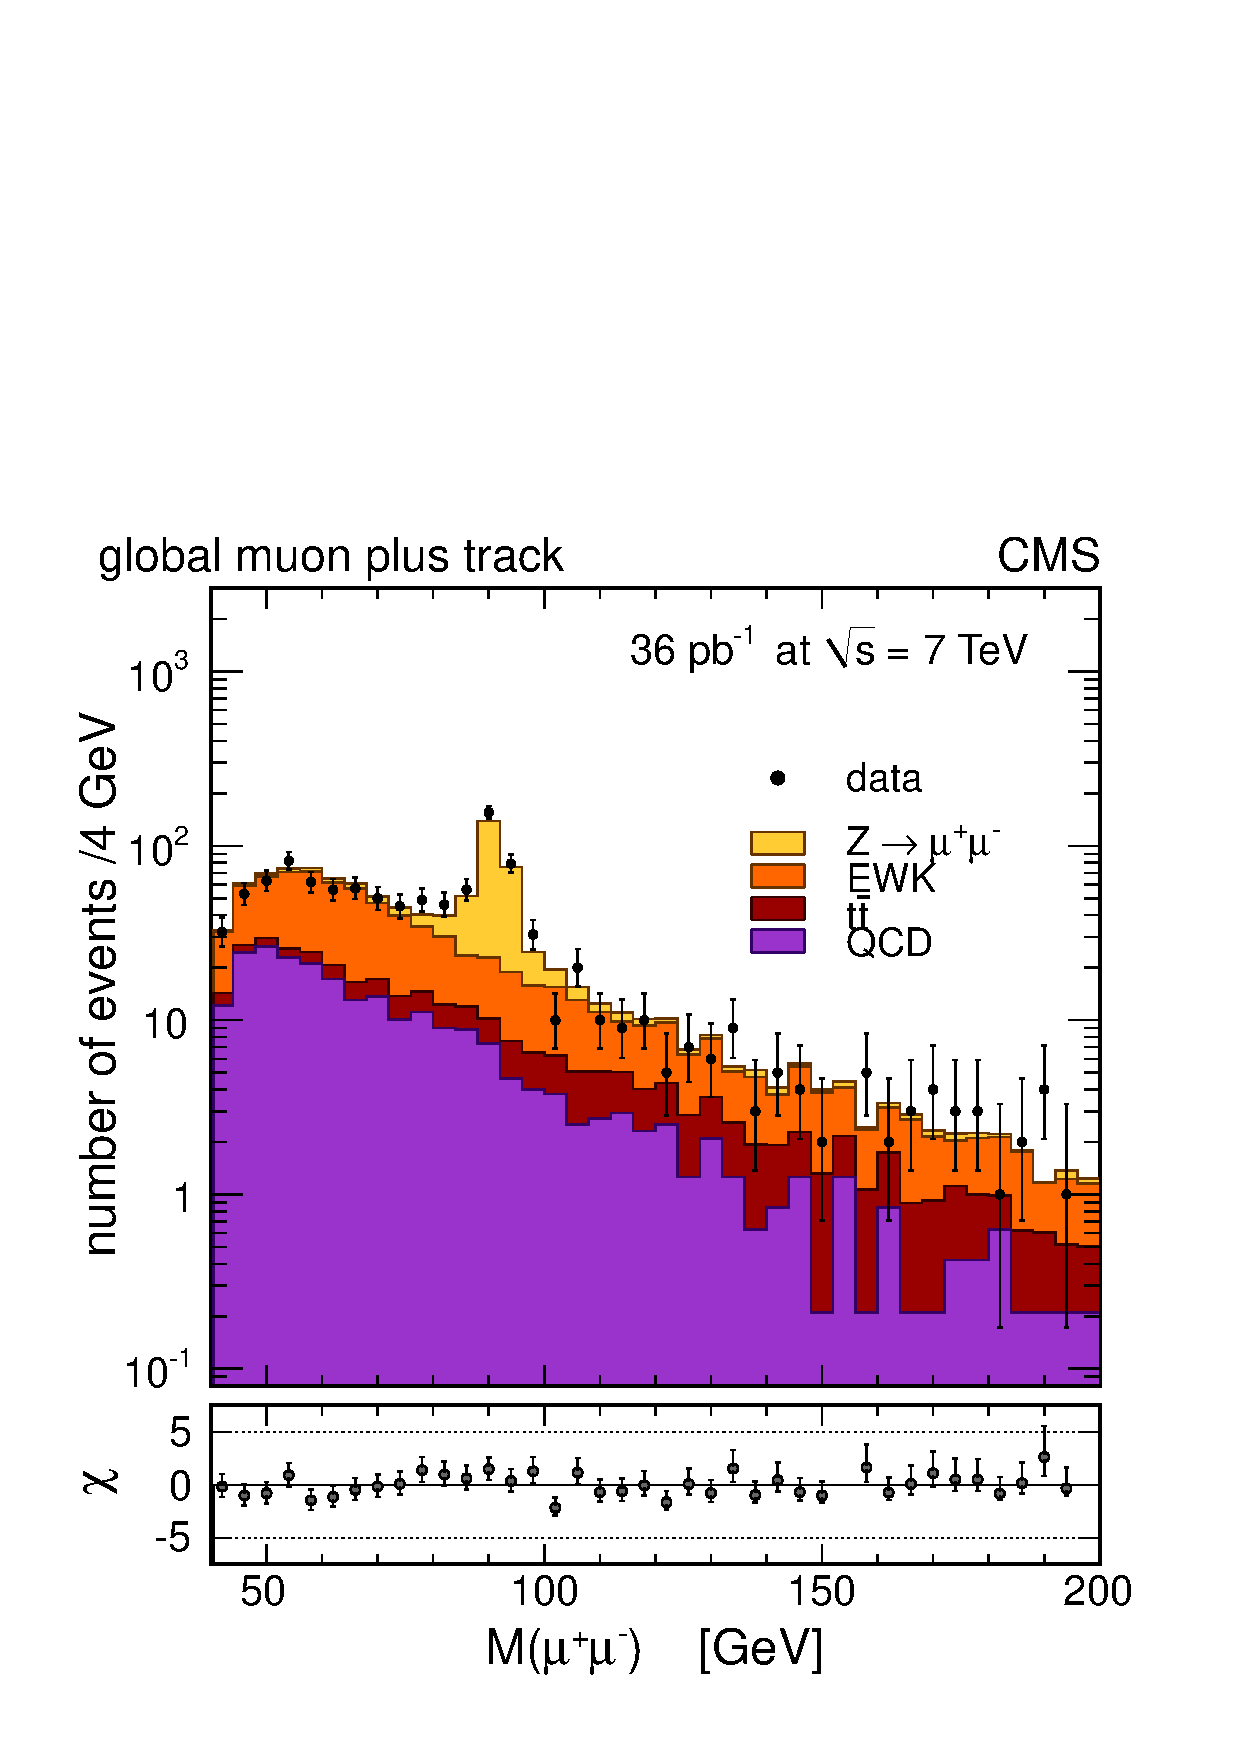
\includegraphics{figs/ZMuTrk_log.pdf}}}
      \end{center}
    \end{minipage}
    \begin{minipage}{73mm}
       \begin{center}
       \resizebox{!}{1.0\textwidth}{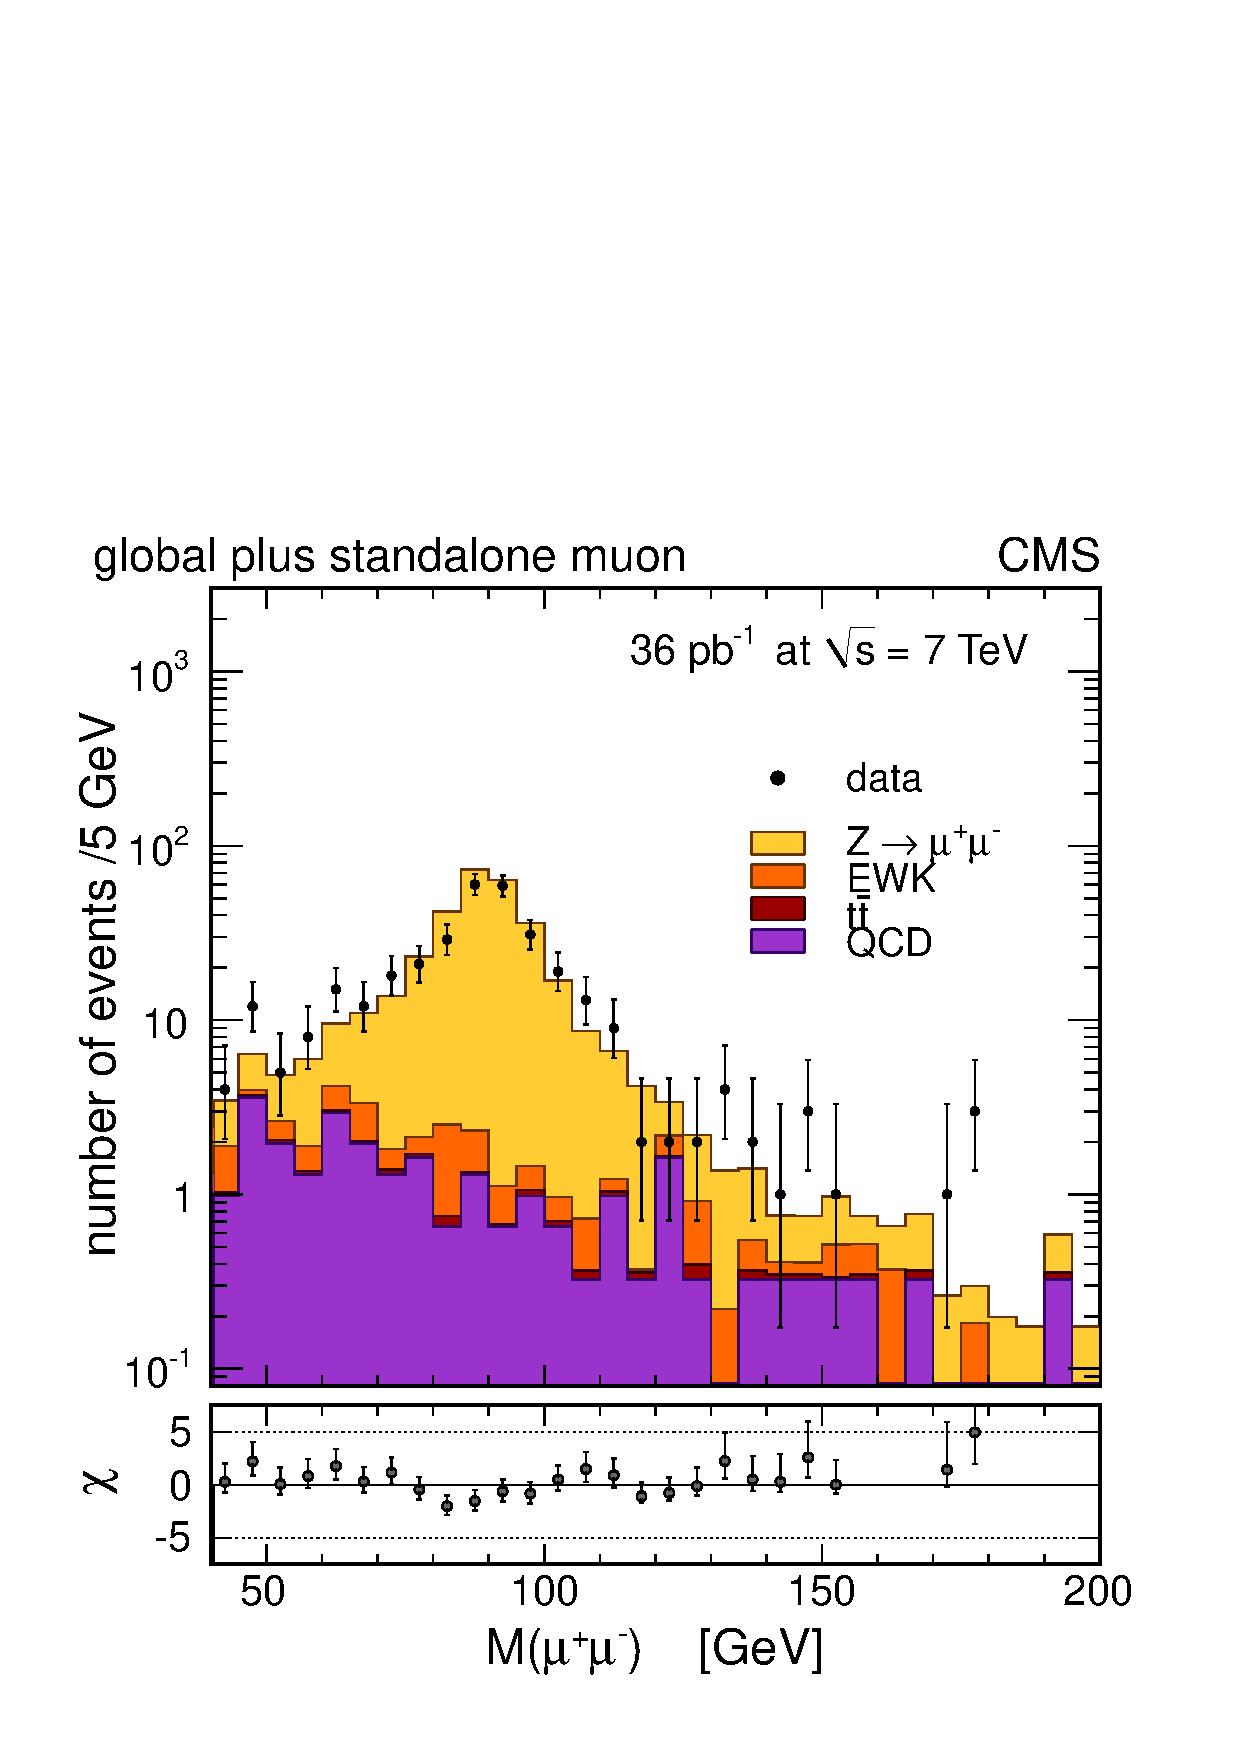
\includegraphics{figs/ZMuSta_log.pdf}}
      \end{center}
    \end{minipage}
\caption{Distributions of the dimuon invariant mass for the selected
$\Zmut$ (left) and $\Zmus$ (right) candidates.
The points with the error bars represent the data.
Superimposed are the expected distributions from simulations, normalized
to an integrated luminosity of $36$~pb$^{-1}$. The expected distributions are
the Z signal (yellow, light histogram), other EWK processes (orange, medium histogram),
$\ttbar$ background (red, dark histogram) and QCD background (violet, black histogram).
}
\label{fig:zNoGold1}
\end{figure}
\begin{figure}[hbtp]
    \begin{center}
     \begin{minipage}{73mm}
       \begin{center}
        \resizebox{!}{1.0\textwidth}{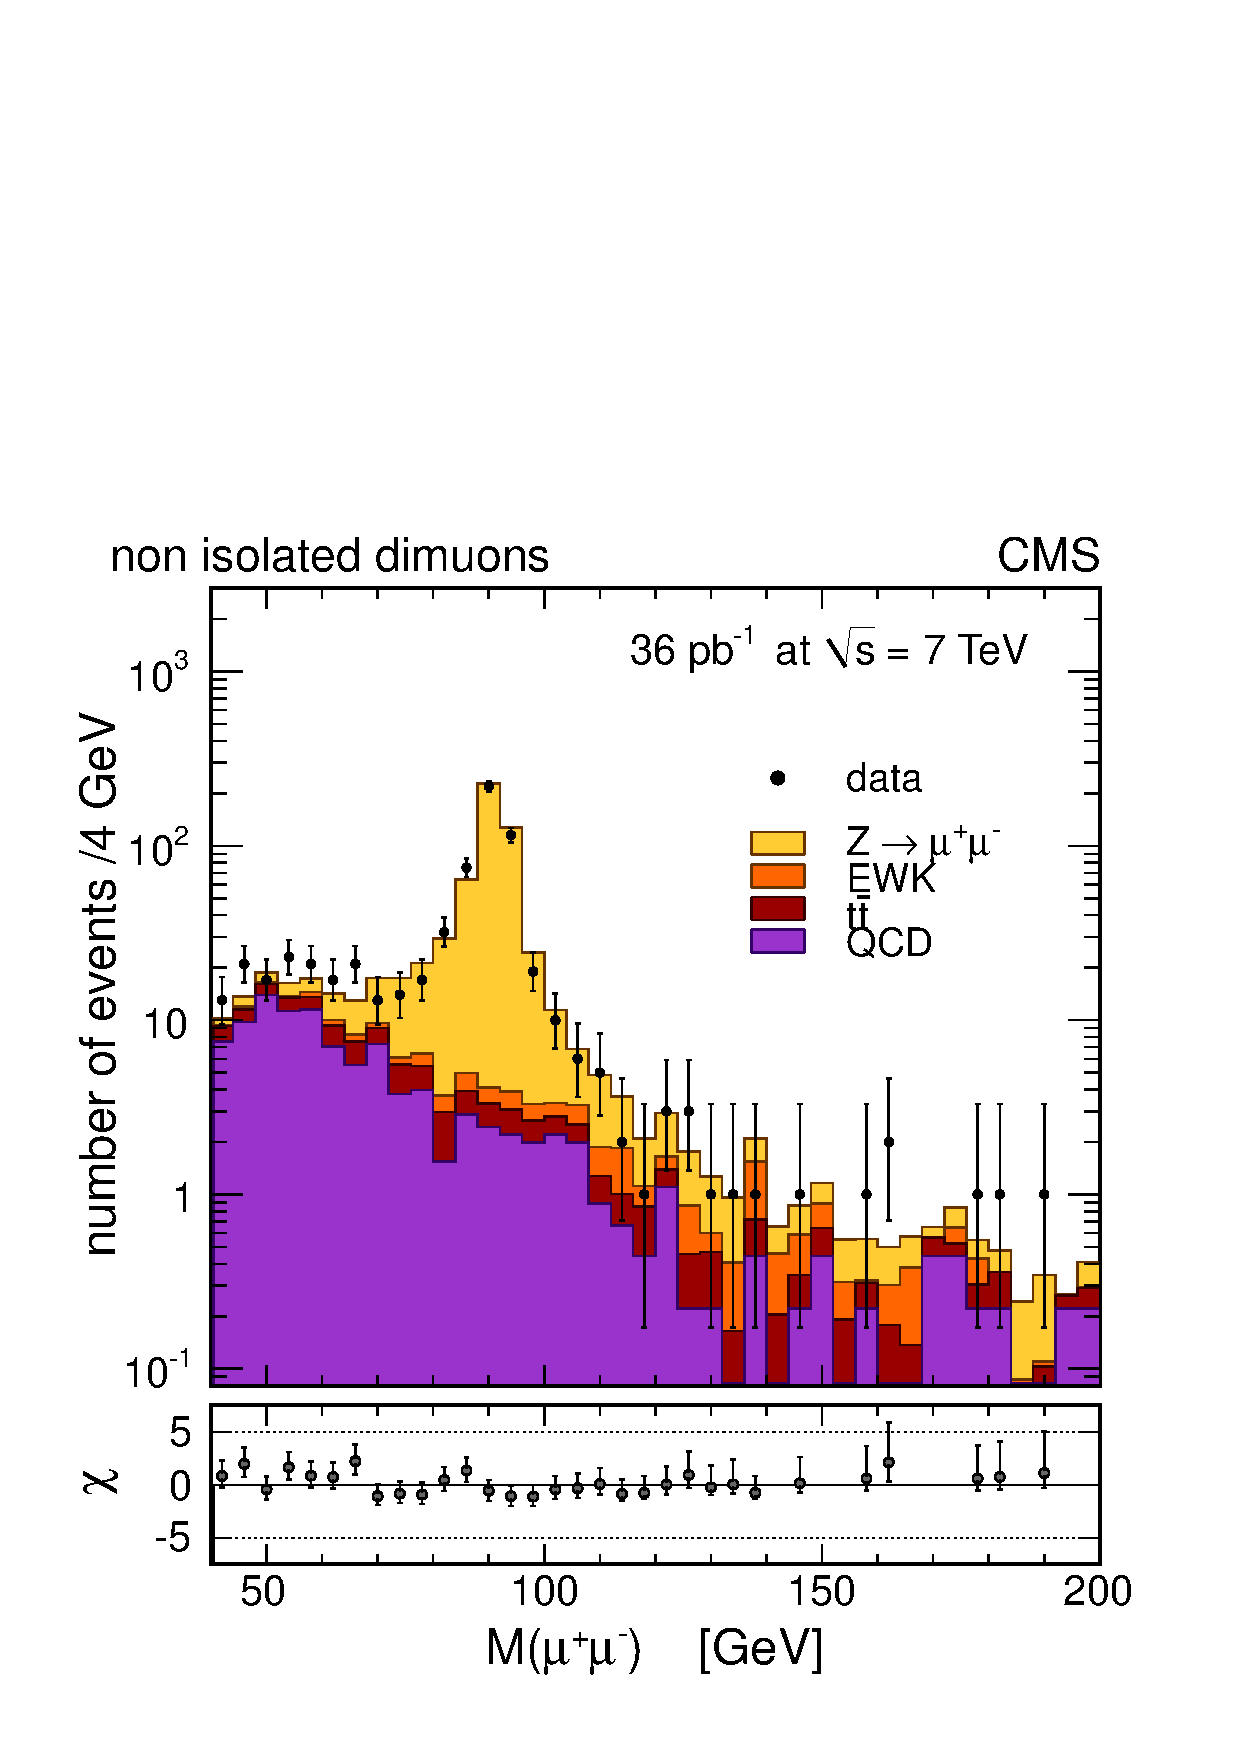
\includegraphics{figs/ZNotIso_log.pdf}}
       \end{center}
     \end{minipage}
   \end{center}
\caption{Distributions of the dimuon invariant mass for the selected
$\ZmumuNonIso$ candidates.
The points with the error bars represent the data.
Superimposed are the expected distributions from simulations, normalized
to an integrated luminosity of $36$~pb$^{-1}$. The expected distributions are
the Z signal (yellow, light histogram), other EWK processes (orange, medium histogram),
$\ttbar$ background (red, dark histogram), and QCD background (violet, black histogram).
}
\label{fig:zNoGold2}
\end{figure}

%, and the background can be considered
%negligible in the 'golden' categories (of the order of few per mille).
% \begin{eqnarray}
%    \NmumuTwoHlt (m) & = & \NmumuTwoHlt f_{peak}(m)\,, \\
%    \NmumuOneHlt (m) & = & \NmumuOneHlt f_{peak}(m)\,, \\
%    \Nmus (m) & = & \Nmus f^s_{peak}(m) + b_{\mu s}(m)\,, \\
%    \Nmut (m) & = & \Nmut f_{peak}(m) + b_{\mu t}(m)\,, \\
%    \NmumuNonIso (m) & = & \NmumuNonIso f_{peak}(m) + b_{\mu\mu}^{\mathrm{non\,iso}}(m)\,. \\
% \end{eqnarray}
The signal-peak distribution can be considered to be identical in the categories
$\Zmumu$ and $\Zmut$  because the momentum resolution in CMS is determined predominantly
by the tracker measurement for muons with $\Pt \leq 200$ GeV.
The binned spectrum of the dimuon invariant mass in the
$\Zmumu$ category, which has the most events of all categories,
is taken as shape model for all categories but $\Zmus$.
The large size of the golden sample ensures that the statistical
uncertainty of the invariant mass distribution has a negligible effect on the cross
section measurement.
The small presence of background is neglected in this distribution.
The uncertainty due to this approximation has been evaluated and
taken as the systematic uncertainty as described in Section~\ref{sec:muonSyst}.

Because only tracker isolation is used, the shape obtained from golden events
can also be used to model the $\ZmumuNonIso$ peak distribution.
A requirement on calorimetric isolation would have distorted the dimuon invariant mass
distribution of events with one nonisolated muon because of FSR,
as has been observed both in simulation and data.

The model of the invariant mass shape for the $\Zmus$ category is also derived from golden dimuon events.
The three-momentum for one of the two muons is taken from only the muon detector track fit,
in order to emulate a stand-alone muon.
To avoid using the same event twice in forming the $\Zmus$ shape model,
the higher-$\Pt$ (lower-$\Pt$) muon is chosen for even (odd) event numbers.

Background shapes are modeled as products of an exponential times a polynomial
whose degree depends on the category.
% :
% \begin{eqnarray}
%   b_{\mu t}(m) & = & N^b_{\mu t} (1 + a_1 m + a_2 m^2) e^{-\alpha m} \\
%   b_{\mu\mu}^{\mathrm{non\,iso}}(m) & = &
%   N_{\mu\mu}^{b\,\,{\mathrm{non\,iso}}} (1 + b_1 m + b_2 m^2) e^{-\beta m} \\
%   b_{\mu s}(m) & = & N^b_{\mu s} (1 + c_1 m + c_2 m^2) e^{-\gamma m}
% \end{eqnarray}
Different background models and different binning sizes are considered for the
categories other than $\Zmumu$ and a systematic uncertainty related to the fitting
procedure is determined accordingly.

%  f_{peak}^{s}(m) & = & \frac{1}{\sqrt{2\pi\sigma_s^2}} e^{-\frac{(m - M)^2}{2 \sigma_s^2} } \\
%The peak function for the $\Zmus$ category, $f_{peak}^{s}(m)$, is modeled as a
%Gaussian, due to the poor resolution, and the low statistics in that sample:

A simultaneous binned fit based on a Poissonian likelihood~\cite{PoisLR} is performed
for the different categories.
%We define, for each category, minus two times the negative logarithmic
%of the following Poissonian likelihood ratio~\cite{PoisLR}:
% \begin{equation}
% \chi^2_{\lambda} = -2 \ln{\lambda(m)} =  -2 \ln{\frac{\mathrm{Poiss}(n_i,
%     \nu_i)}{\mathrm{Poiss}(n_i, n_i)}} = \sum_{i=1}^{n_{\mathrm{bins}}} \nu_i - n_{i} + n_i \log{\frac{n_i}{\nu_i}}\,,
% \end{equation}
% where $\nu_i$ is the expected number of events in the $i^{\mathrm{th}}$-bin in $m$,
% $n_i$ is the measured number of events in that
% bin, and $\mathrm{Poiss}(n,\nu)$ is a Poissonian distribution.
% The simultaneous fit is performed minimizing the sum $R$ of the five $\chi^2_\lambda,j$ from
% the different categories $j=1,\cdots, 5$, i.e.:
% \begin{equation}
% R =  \sum_{j=1}^{5} \chi^2_{\lambda,j}   = 2  \sum_{j=1}^{5} \sum_{i=1}^{n_{\mathrm{bins}}^{(j)}} \nu^{(j)}_i - n^{(j)}_{i} + n^{(j)}_i \log{\frac{n^{(j)}_i}{\nu^{(j)}_i}}\,.
% \label{eq:PoisLR}
% \end{equation}
% For sufficiently large $\nu_i$, as in our case, the minimum of $R$ follows with good approximation a $\chi^2$ distribution,
% allowing a goodness-of-fit test.
% Using only the number of events for the two categories with the largest statistics,
% $\ZmumuTwoHlt$ and $\ZmumuOneHlt$, the Z yield and the four efficiencies can be obtained minimizing the
% following expression, which can be obtained from Eq.~\ref{eq:PoisLR} using a single bin in the Gaussian approximation for $\ZmumuTwoHlt$
% and $\ZmumuOneHlt$:
% \begin{eqnarray*} \label{chi2}
% R & = &
% \frac{(\NmumuTwoHlt - \NZtomumu\effHlt^2\effIso^2\effTrk^2\effSa^2)^2}{\NmumuTwoHlt} +  \\
% & & \frac{(\NmumuOneHlt - 2\NZtomumu\effHlt(1-\effHlt)\effIso^2\effTrk^2\effSa^2)^2}{\NmumuOneHlt} +  \\
% & & \chi^2_{\lambda, \mu s} +
% \chi^2_{\lambda, \mu t} +
% \chi^{\nonIso\,\, 2}_{\lambda, \mumu}\, ,
% \end{eqnarray*}
% where we use the event counts only in the  $\ZmumuOneHlt$ and $\ZmumuTwoHlt$ 'golden'
% categories and the Poissonial terms $\chi^2_{\lambda, \mu s}$, $\chi^2_{\lambda, \mu t}$ and
% $\chi^{\nonIso\,\, 2}_{\lambda, , \mumu}$ for the remaining categories.
% The likelihood ratio fit is equivalent to an ordinary $\chi^2$
% for sufficiently large statistics and we verified that, with the current data sample,
% it gives the same central value and statistical uncertainty.
%We perform the fit in the range $60 < m < 120~\mathrm{GeV}/c^2$.
%Full details on the signal and background modeling assumptions and
%correlation studies are present in~\cite{CMS_AN_2010-345}.
Table~\ref{fig:fitRes_36pb} reports the signal yield and single-muon efficiencies determined from
the simultaneous fit and the ratios of the fitted to simulation efficiencies.
A goodness-of-fit test gives a probability ($p$-value) of 0.36 for this fit.

%The resulting fit $p$-value shows the good quality of the fit.
%With the analyzed statistics, a second degree polynomial function is
%taken for modeling  the background shape.

\begin{table}[htbp] %L.L.
\begin{center}
\caption{Signal yield and efficiencies determined from data with the simultaneous fit, and
  ratios of efficiencies determined from the fit and the simulation.}
\label{fig:fitRes_36pb}
\begin{tabular}{|c|c|c|}
\hline
Quantity & Fit results from data & Data/simulation\\
\hline\hline
$\NZtomumu$ &13\,728 $\pm$ 121   & \\
\hline
$\effHlt$ & 0.9203 $\pm$ 0.0019  &0.9672 $\pm$ 0.0020   \\
$\effIso$ & 0.9813 $\pm$ 0.0010& 0.9962 $\pm$  0.0011 \\
$\effSa$ & 0.9762  $\pm$ 0.0012 & 0.9964 $\pm$ 0.0013 \\
$\effTrk$ & 0.9890 $\pm$ 0.0006  & 0.9949 $\pm$ 0.0007  \\
\hline
\end{tabular}
\end{center}
\end{table}

%In order to correct the fitted yield $\NZtomumu$ for the presence of background,
%the estimated irreducible background fraction is subtracted.
%$f_{bkg}=0.44 \pm 0.02\%$.

The background in the $\Zmumu$ golden category (of the order of few per mille)
was neglected in the fit. In order to correct the fitted yield $\NZtomumu$ for
the presence of this background, we subtract the small estimated irreducible
background fraction.

A $(1.0\pm 0.5)\%$ overall efficiency correction due to the loss of muon events because of trigger
prefiring is also applied (Section~\ref{sec:muonEff}).

The estimated cross section is $968\pm 8 \mathrm{(stat.)}$~pb.

As cross-check, a simpler analysis based on event counting was also performed.
The same selection was applied, and the number of events with two global muon, reported
in Sec~\ref{sec:muonid}, was used as signal yield. 
The signal yield was then corrected for the relevant efficiencies that have 
been evaluated with a \TNP method in a single $\Pt$ and $\eta$ bin, resulting in a
cross section estimate of $969\pm 8 \mathrm{(stat.)}$~pb, in good agreement
with the simultaneous fit method.
